\documentclass{article}
\usepackage[utf8]{inputenc}
\usepackage{indentfirst}
\usepackage{graphicx}
\usepackage[margin =1.0in]{geometry}
\usepackage{amsmath,amsthm,amsfonts}
\usepackage[linesnumbered,ruled]{algorithm2e}
\usepackage[backend=bibtex, style=authoryear]{biblatex}
\usepackage{listings}

\usepackage[usenames,dvipsnames]{color}    

\lstset{ 
  language=R,                     % the language of the code
  basicstyle=\ttfamily, % the size of the fonts that are used for the code
  numbers=left,                   % where to put the line-numbers
  numberstyle=\tiny\color{Blue},  % the style that is used for the line-numbers
  stepnumber=0,                   % the step between two line-numbers. If it is 1, each line
                                  % will be numbered
  numbersep=5pt,                  % how far the line-numbers are from the code
  backgroundcolor=\color{white},  % choose the background color. You must add \usepackage{color}
  showspaces=false,               % show spaces adding particular underscores
  showstringspaces=false,         % underline spaces within strings
  showtabs=false,                 % show tabs within strings adding particular underscores
  %frame=single,                   % adds a frame around the code
  rulecolor=\color{black},        % if not set, the frame-color may be changed on line-breaks within not-black text (e.g. commens (green here))
  tabsize=2,                      % sets default tabsize to 2 spaces
  captionpos=b,                   % sets the caption-position to bottom
  breaklines=true,                % sets automatic line breaking
  breakatwhitespace=false,        % sets if automatic breaks should only happen at whitespace
  keywordstyle=\color{RoyalBlue},      % keyword style
  commentstyle=\color{YellowGreen},   % comment style
  stringstyle=\color{ForestGreen}      % string literal style
} 


\graphicspath{{/Users/benjamindraves/Desktop/figures/}}
\lstset{inputpath = /Users/benjamindraves/Desktop/Latent-Network-Models/Code/GoT/}

\setlength\bibitemsep{1.5\itemsep}
\bibliography{ref.bib}

\title{Computational Techniques in Latent Network Models}
\author{Lily Chou, Ben Draves, Nathan Josephs, Kelly Kung}
\date{December 12, 2018}

\begin{document}

\maketitle

\section{Introduction}

\textit{Game of Thrones} is a popular HBO TV series adapted from George R.R. Martin's best-selling book series \textit{A Song of Ice and Fire}. The medieval fantasy epic describes the stories of powerful families - kings and queens, knights and renegades, liars and honest men - playing a deadly game for control of the Seven Kingdoms of Westeros and to sit atop the Iron Throne. Conspiracy and deception, power and exile, blood and tears run through the plot, sewing together characters with various backgrounds including royals and peasants, as well as ice zombies and dragons. As the plot develops with each book release, readers wonder where the storyline leads. Within the Seven Kingdoms, enemies become friends and vice-versa, all the while winter spreads as the battle of ice and far draws nearer. We want to keep track of the dynamics between characters as the plots develops. Some may keep a leaf diagram between characters; here we propose an alternative -- let the data do the work.

After discovering a dataset on the exchanges between the characters from the third book, \textit{A Storm of Swords}, we start to wonder if, and what, information we can extract. In particular, how can we make inferences on the clustering of the characters. To address this, we turn to research of Peter Hoff on latent network models. In Section \ref{Data}, we show how the relationships between characters from the book naturally arise as a network. Before fitting a model, we explain the latent network model framework in Section \ref{Models}. We then present two methods for fitting our model in Section \ref{Computational Methods} and then compare the results of the two methods in Section \ref{Results}. Finally, in Section \ref{Conclusion} we end with a discussion on the implications of our findings, as well as possible future work. We provide our code in the Appendix.

\section{Data}\label{Data}
Due to its global fame, \textit{Game of Thrones} has been studied in many different contexts, especially in network analysis. Therefore, there are many readily available datasets. In our project, we use the dataset from \cite{beveridge2016network}, which contains information about characters' interactions in the third book of the series. In this case, an \textit{interaction} occurs if the characters' names appear within fifteen words of one another. This could mean that the characters interacted with each other, conversed with each other, or were generally mentioned together by another means. There is also a column that contains the number of times each pair interacts with one another. Using this dataset, we constructed a weighted network using the number of interactions as weights. Here, the nodes represent the characters and the edges represent the interactions. We use an adjacency matrix, $A$, to represent the network, where the $a_{i,j}$ element represents the number of times the characters interacted with each other. Note that this means if $a_{i.j} = 0$, there are no recorded interactions between character $i$ and $j$ based on how an \textit{interaction} is defined. Although the original dataset is intended as a directed network, we treat it as an undirected network in order to simplify our models.

After transforming the dataset, our network $G$ contains $N_V(G) = 107$ nodes and $N_E(G) = 352$ edges which means it is quite sparse since it only contains approximately $6.20\%$ of $\binom{N_V(G)}{2} = 5,671$ possible edges. Figure \ref{filtered_net} shows the network described. 
\begin{figure}[h]\label{filtered_net}
	\centering
	\vspace*{-3cm}
	\hspace*{-4cm}
	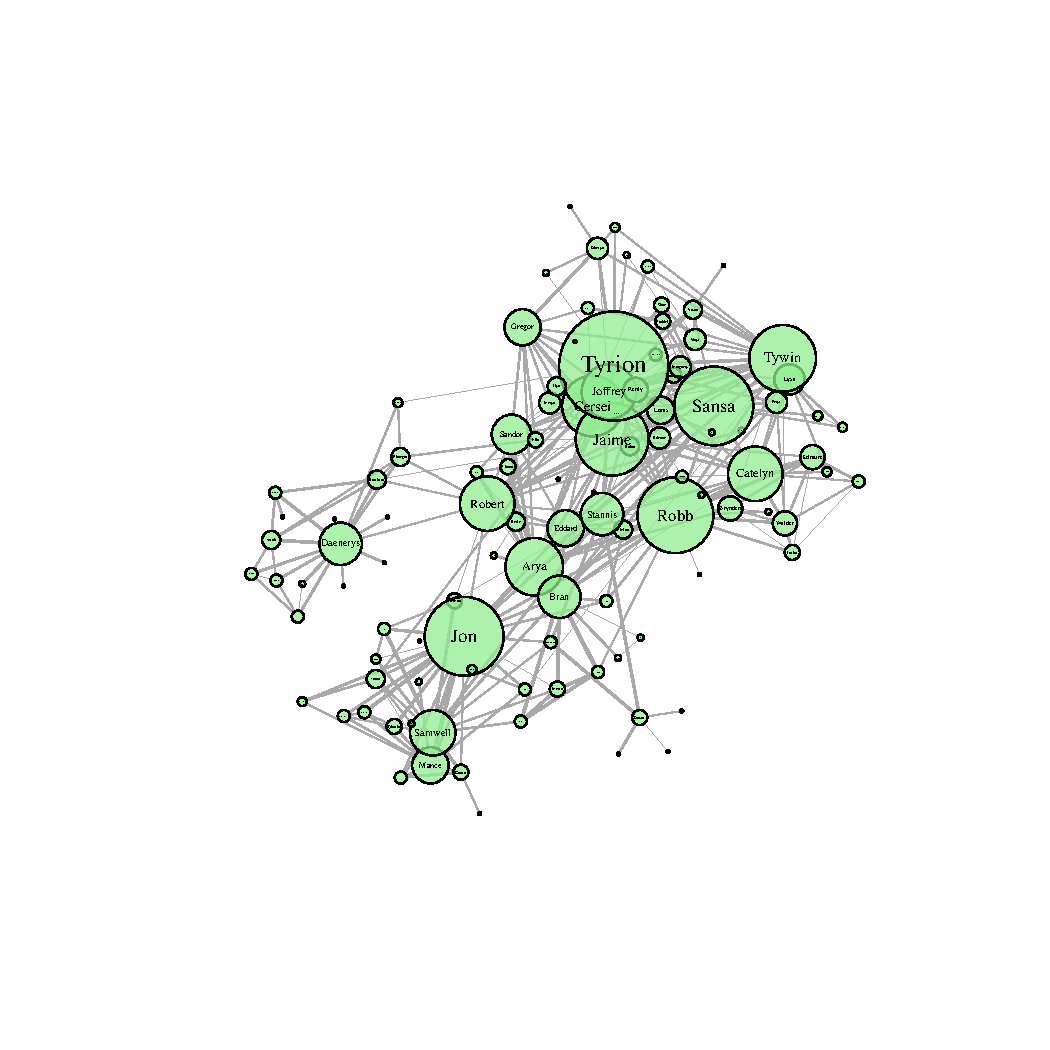
\includegraphics[width = .5\textwidth, height = 5in]{initial_net.pdf}
	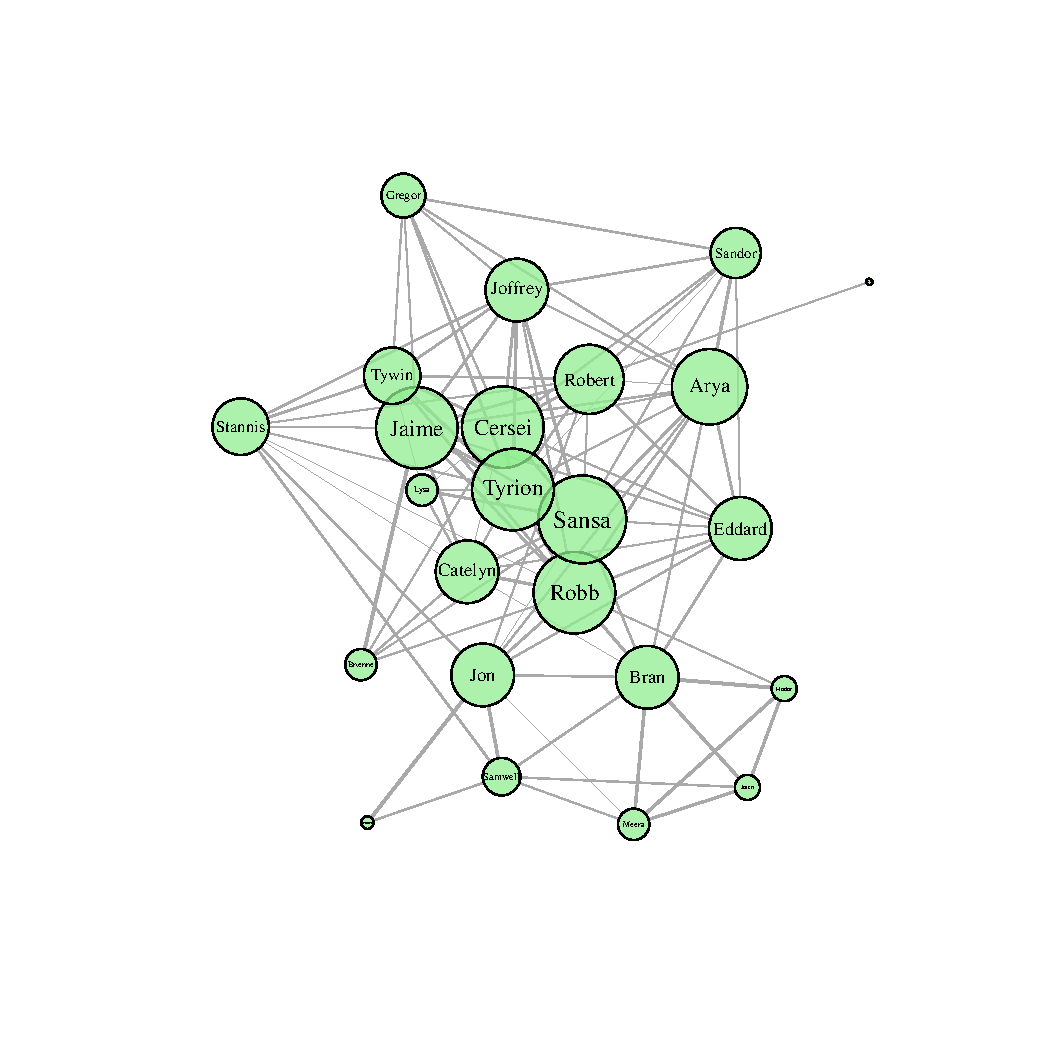
\includegraphics[width = .5\textwidth, height = 5in]{filtered_net.pdf}
	\hspace*{-4cm}
	\vspace*{-2cm}
\end{figure}
In order to account for the sparsity of our network, we consider a subnetwork which only contains pairs of characters with at least 100 interactions. We chose a cutoff of 100 interactions because we want to focus our analysis on only the main characters. Looking at the distribution of the weighted degree, we see that $77.6\%$ of the characters had fewer than 100 interactions. Therefore, it makes sense to use this cutoff to limit our analysis to only the main characters. By doing so, our new network $G'$ contains $N_V(G') = 24$ nodes and $N_E(G') = 102$ edges. Here, we see that the network now contains $38.2\%$ of 276 possible edges, which is a more appropriate level of density for our analysis. Everything that follows is done on this subnetwork $G'$. Figure \ref{filtered_net} shows this subnetwork $G'$, and indeed, we recognize the main characters remain in our network.

\section{Models} \label{Models}


\subsection{Model Formulation}\label{Model Formulation}

A modern and popular class of network models is the \textit{Latent Network Model}. This model, first introduced by \cite{Hoff2002}, associates each vertex $v\in V$ with a latent variable $Z_v\in \mathcal{V}$. Using these variables, the probability of an $E_{ij}$ being in the network is given by $p_{ij} = \kappa(Z_i, Z_j)$ where $\kappa:\mathcal{V}\times\mathcal{V}\to[0,1]$. Following this work, the authors extend these models to the mixed-model, regression framework where nodal attribute vectors $x_V$ are used in modeling the probability of an edge presense (\cite{KRIVITSKY2009204}). For simplicity we do not consider nodal attributes in this work and instead focus our inference on the latent variables associated with each network. Formally, we model the presence of an edge given our latent variables as
\[\text{logit} \ \mathbb{P}(Y_{ij} = 1|Z) = ||Z_i - Z_j|| + \epsilon_{ij}\]
where
\[Z_i \overset{ind}{\sim}\sum_{k=1}^G \lambda_k\text{MVN}_d(\mu_k,\sigma_k^2I_d)\]
Putting priors over $\mu_k$ and  $\sigma_k^2$, as well as introducing the latent variable $K$ representing the group from which $Z$ is drawn, we have the following model formulation:

\begin{align*}
Y_{ij} | Z_i, Z_j &\overset{ind}\sim \text{Bern}\Big[\text{logit}^{-1}\big(\Vert Z_i - Z_j \Vert\big)\Big] \\
Z_i | K_i = k_i &\overset{ind}\sim MVN(\mu_{k_i}, \sigma_{k_i}^2 I_d) \\
K &\overset{iid}\sim \text{Multinoulli}\big(G, \lambda \big) \\
\lambda_k &\overset{iid}\sim \frac{1}{G} \\
\mu_k &\overset{iid}\sim \text{MVN}_d(0, I_d) \\
\sigma_k^2 &\overset{iid}\sim \text{Inv} \chi^2_1
\end{align*}
With these, we can write the complete likelihood which we will use in both our fitting procedures. We let $\theta = (\mu, \sigma^2, K, \lambda)$ denote our nuisance parameters. Then, we have

\begin{align*}
\mathcal{L}(Z, \theta; Y) &= \prod_{i<j}\mathbb{P}(Y_{ij} | Z_i, Z_j) \mathbb{P}(Z_i | K_i, \mu_{k_i}, \sigma_{k_i}^2) \mathbb{P}(Z_j | K_j, \mu_{k_j}, \sigma_j^2) \\ 
&\ \ \ \ \ \ \ \ \times  \mathbb{P}(K_i | \lambda_i) \mathbb{P}(\lambda_i)\mathbb{P}(\mu_{k_i})\mathbb{P}(\sigma_{k_i}^2)\mathbb{P}(K_j)\mathbb{P}(\mu_{k_j})\mathbb{P}(\sigma_{k_j}^2) \\
&= \prod_{i<j}\Big(\text{logit}^{-1}\big(\Vert Z_i-Z_j\Vert)\Big)^{Y_{ij}}\Big(1 - \text{logit}^{-1}\big(\Vert Z_i-Z_j\Vert)\Big)^{1 - Y_{ij}} \\
&\ \ \ \ \ \ \ \ \times f_{{MVN}_d} (\mu_{k_i}, \sigma_{k_i}^2I_d)\times\lambda_i \times \frac{1}{G} \times f_{{MVN}_d} (0, I_d) \times f_{\text{Inv}\chi^2_2} \\
&\ \ \ \ \ \ \ \ \times f_{{MVN}_d}(\mu_{k_j}, \sigma_{k_j}^2I_d)\times  \lambda_j \times \frac{1}{G} \times f_{{MVN}_d} (0, I_d) \times f_{\text{Inv}\chi^2_2} \\
&\propto \prod_{i<j}\Big(\text{logit}^{-1}\big(\Vert Z_i-Z_j\Vert)\Big)^{Y_{ij}}\Big(1 - \text{logit}^{-1}\big(\Vert Z_i-Z_j\Vert)\Big)^{1 - Y_{ij}} \\
&\ \ \ \ \ \ \ \ \times \frac{1}{(\sigma_{k_i}^2)^{1/2}}\exp\Big\{-\frac{1}{2\sigma_{k_i}^2}(Z_i - \mu_{k_i})^T( Z_i - \mu_{k_i}) \Big\} \enspace \frac{1}{(\sigma_{k_j}^2)^{1/2}}\exp\Big\{-\frac{1}{2\sigma_{k_j}^2}(Z_j - \mu_{k_j})^T (Z_j - \mu_{k_j})\Big\} \\
&\ \ \ \ \ \ \ \ \times \exp\Big\{-\frac{1}{2}\mu_{k_i}^T\mu_{k_i}\Big\}\exp\Big\{-\frac{1}{2}\mu_{k_j}^T\mu_{k_j}\Big\}  \times \frac{1}{(\sigma_{k_i}^2)^2}\exp\Big\{-\frac{1}{\sigma_{k_i}^2}\Big\}\frac{1}{(\sigma_{k_j}^2)^2}\exp\Big\{-\frac{1}{\sigma_{k_j}^2}\Big\} \times \lambda_i \times \lambda_j
\end{align*}


%Hence the log-likelihood, up to a constant, is
%\begin{align*}l(Z, \theta ; Y) &\overset{c}= \sum_{i<j} \Big\{Y_{ij} \Vert Z_i - Z_j \Vert - \log \big(1 + \exp\big(\Vert Z_i - Z_j\Vert\big)\big)\Big\} \\&\ \ \ \ \ \ \ \ - \log \sigma_{k_i} - \frac{1}{2\sigma_{k_i}^2}(Z_i - \mu_{k_i})^T( Z_i - \mu_{k_i}) - \log \sigma_{k_j} - \frac{1}{2\sigma_{k_j}^2}(Z_j - \mu_{k_j})^T (Z_j - \mu_{k_j})  \\&\ \ \ \ \ \ \ \ -\frac{1}{2}\Big(\mu_{k_i}^T\mu_{k_i} + \mu_{k_j}^T\mu_{k_j} + \sigma_{k_i}^2 + \sigma_{k_j}^2\Big)  + \log \lambda_i + \log \lambda_j\end{align*}


%&\ \ \ \ \ \ \ \ - \frac{1}{2}\log 2\pi - \frac{1}{2}\log \sigma_k^2 - \frac{(Z_i - \mu_k)^2}{2\sigma_k^2}  - \frac{1}{2}\log 2\pi - \frac{1}{2}\log \sigma_j^2 - \frac{(Z_j - \mu_j)^2}{2\sigma_j^2} \\
%&\ \ \ \ \ \ \ \ - \log G - \log G \\
%&\ \ \ \ \ \ \ \ - \frac{1}{2} \log \big(2\pi\det(I_2)\big) - \frac{1}{2}(\mu_k^TI_2^{-1}\mu_k) - \frac{1}{2} \log \big(2\pi\det(I_2)\big) - \frac{1}{2}(\mu_j^TI_2^{-1}\mu_j) \\
%&\ \ \ \ \ \ \ \ - \frac{1}{2}\log 2 - \log \Gamma(\frac{1}{2}) - \frac{1}{2}\log \sigma_k^2 - \frac{\sigma_k^2}{2} - \frac{1}{2}\log 2 - \log \Gamma(\frac{1}{2}) - \frac{1}{2}\log \sigma_j^2 - \frac{\sigma_j^2}{2} \\
%&\overset{c}= \text{simplified up to constant}

%Below we write $\mathcal{L}_1$, $\ell_1$ are likelihood methods for the unweighted network model. If we wish to include the weights into our modeling procedure, we construct a second log-likelihood $\ell_2$. 
%\begin{align}
%\mathcal{L}_1(\mathbf{Z}; \mathbf{Y}) &= \prod_{i<j} \left\{\text{logit}^{-1}(||Z_i - Z_j||)\right\}^{Y_{ij}}\left\{1-\text{logit}^{-1}(||Z_i - Z_j||)\right\}^{1-Y_{ij}}\\
%\ell_1(\mathbf{Z};\mathbf{Y}) &=  \sum_{i<j}Y_{ij}||Z_i - Z_j|| - \log\left(1 + \exp\left(||Z_i - Z_j||\right)\right)\\ 
%\ell_2(\mathbf{Z}; \mathbf{Y}) &= \sum_{i<j}y_{ij}(||Z_i - Z_j||) - \exp(||Z_i - Z_j||) - \log(y_{ij})\\
%\end{align}

\section{Computational Methods} \label{Computational Methods}

\subsection{EM}
One method for finding the latent variables $Z_i$ for each node is the Expectation-Maximization (EM) algorithm. Unfortunately, the likelihood given in Section \ref{Model Formulation} cannot easily be handled with EM. In particular, finding $\mathbb{E}_{Z_i, Z_j | Y, \theta}\Big[l(Z, \theta ; Y)\Big]$ is difficult. One solution is to sample and use Monte Carlo methods to estimate the expectation in the E-step and then proceed with the M-step. This is the so-called Monte Carlo EM (MCEM) method. 

Instead, we simplify our model to make EM more analytically tractable. In Section \ref{MCMC}, we fit the full model using MCMC. Here, we fit two simplified models: an unweighted model where $Y$ indicates the presence of an edge and a weighted model where now $Y$ represents the number of interactions between characters.

\subsubsection{Unweighted Model}
We first fit an unweighted model on the presence of an edge in the network, which is defined by:

\begin{align*}
Y_{ij} | p_{ij} &\overset{ind}\sim \text{Bern}(p_{ij}) \\
p_{ij} &\overset{iid}\sim \text{Beta}(\alpha, \beta)
\end{align*}
where we define $p_{ij} \equiv 2-2*\text{logit}^{-1} (d_{ij}) $ where $d_{ij}$ are latent distances defined in Section \ref{Model Formulation} and are calculated by $d_{ij} = logit(1 - \frac{p_{ij}}{2})$. We define $p_{ij}$ in this manner to ensure that an infinite distance results in zero probability of interaction and a distance of zero results in a probability of one. Then the likelihoods are 

\begin{align*}
\mathcal{L}(p, \alpha, \beta; Y) &= \prod_{i<j}p_{ij}^{Y_{ij}}\big(1 - p_{ij}\big)^{1 - Y_{ij}} \frac{\Gamma(\alpha + \beta)}{\Gamma(\alpha)\Gamma(\beta)}p_{ij}^{\alpha - 1}\big(1-p_{ij}\big)^{\beta - 1} \\
l(p, \alpha, \beta ; Y) &= \sum_{i<j} Y_{ij}\log \Big(\frac{p_{ij}}{1 - p_{ij}}\Big) + \log(1-p_{ij})  \\
&\ \ \ \ \ \ \ \ + \log \Gamma(\alpha + \beta) - \log \Gamma(\alpha) - \log \Gamma(\beta) \\
&\ \ \ \ \ \ \ \ + (\alpha - 1)\log p_{ij} + (\beta - 1)\log(1 - p_{ij})
\end{align*}

%Gamma
%\begin{align*}
%\mathcal{L}(d_{ij}, \alpha, \beta; Y) &= \prod_{i<j}\Big(\text{logit}^{-1}\big(d_{ij})\Big)^{Y_{ij}}\Big(1 - \text{logit}^{-1}\big(d_{ij})\Big)^{1 - Y_{ij}} \\
%&\ \ \ \ \ \ \ \ \times \frac{\beta^\alpha}{\Gamma(\alpha)}d_{ij}^{\alpha - 1}\exp\big\{-\beta d_{ij}\big\} \\
%l(d_{ij}, \alpha, \beta ; Y) &= \sum_{i<j} Y_{ij}d_{ij} - \log \big(1 + \exp\big(d_{ij}\big)\big) \\
%&\ \ \ \ \ \ \ \ + \alpha \log \beta - \log \Gamma(\alpha) + (\alpha - 1) \log d_{ij} - \beta d_{ij}
%\end{align*}


For the E-step, we observe that the beta distribution is conjugate to the binomial and since $p_{ij}$ only depends on the data through $Y_{ij}$, we have the following likelihood. Note we just suppress our parameters $\theta = \{\alpha, \beta\}$.

\begin{align*}
p_{ij} | Y_{ij}, \theta &\propto \text{Bern}(p_{ij})\times \text{Beta}(\alpha, \beta)\\
&= \text{Beta}\Big(\alpha + Y_{ij}, \beta + 1 - Y_{ij}\Big)
\end{align*}
Therefore, we have
\begin{align*}
%\pi_{ij} &\equiv \mathbb{E}_{p_{ij} | Y_{ij}, \theta} [p_{ij}] = \frac{\alpha + Y_{ij}}{\alpha + \beta + 1} \\
\pi_{ij} &\equiv \mathbb{E}_{p_{ij} | Y_{ij}, \theta} \big[\log p_{ij}\big] = \Psi\Big(\alpha + Y_{ij}\Big) - \Psi\Big(\alpha + \beta + 1\Big) \\
\eta_{ij} &\equiv \mathbb{E}_{p_{ij} | Y_{ij}, \theta} \big[\log (1 - p_{ij})\big] = \Psi\Big(\beta + 1 - Y_{ij}\Big) - \Psi\Big(\alpha + \beta + 1\Big)
\end{align*}
where $\Psi$ is the digamma function. Thus
\begin{align*}
Q\big(\theta; \theta^{(t)}\big) &\equiv \mathbb{E}_{p | Y, \theta^{(t)}} \Big[l(p; Y, \theta)\Big] \\
&= \sum_{i<j} (Y_{ij} + \alpha - 1) \mathbb{E}_{p_{ij} | Y_{ij}, \theta^{(t)}} [\log  p_{ij}] + (\beta -Y_{ij}) \mathbb{E}_{p_{ij} | Y_{ij}, \theta^{(t)}} \big[\log (1-p_{ij})\big] \\
&\ \ \ \ \ \ \ \ + \log \Gamma(\alpha + \beta) - \log \Gamma(\alpha) - \log \Gamma(\beta) \tag{E}
\end{align*}



For the M-step, we simply take the partial derivatives of $Q\big(\theta; \theta^{(t)}\big)$ with respect to $\alpha$ and $\beta$. Note that we will need an approximate solution in both cases since the digamma function prevents us from finding an analytic solution. For this, we use the Newton-Raphson Method.

\begin{align*}
\frac{\partial Q\big(\theta; \theta^{(t)}\big)}{\partial \alpha^{(t)}} &= \sum_{i<j} \mathbb{E}_{p_{ij} | Y_{ij}, \theta^{(t)}} \big[\log p_{ij}\big] + \Psi\Big(\alpha^{(t+1)} + \beta^{(t)}\Big) - \Psi(\alpha^{(t+1)})= 0 \\
&\implies \Psi\Big(\alpha^{(t+1)} + \beta^{(t)}\Big) - \Psi(\alpha^{(t+1)}) = -\frac{\sum_{i<n}\mathbb{E}_{p_{ij} | Y_{ij}, \theta^{(t)}} \big[\log p_{ij}\big]}{{n \choose 2}} \tag{MU1} \\
\frac{\partial Q\big(\theta; \theta^{(t)}\big)}{\partial \beta^{(t)}} &= \sum_{i<j} \mathbb{E}_{p_{ij} | Y_{ij}, \theta^{(t)}} \big[\log (1- p_{ij})\big] + \Psi\Big(\alpha^{(t+1)} + \beta^{(t+1)}\Big) - \Psi(\beta^{(t+1)}) = 0 \\
&\implies \Psi\Big(\alpha^{(t+1)} + \beta^{(t+1)}\Big) - \Psi(\beta^{(t+1)}) = -\frac{\sum_{i<n}\mathbb{E}_{p_{ij} | Y_{ij}, \theta^{(t)}} \big[\log (1 - p_{ij})\big]}{{n \choose 2}} \tag{MU2} \\
\end{align*}

For the Newton-Raphson Method, we first define 
\begin{align*}
g(\alpha) &= \Psi \big(\alpha + \beta^{(t)} \big) - \Psi(\alpha) + \sum_{i < j}\frac{ \mathbb{E}_{p_{ij} | Y_{ij}, \theta^{(t)}} \big[\log p_{ij}\big] }{{n \choose 2}} \\
&\implies g'(\alpha) = \Psi' \big(\alpha + \beta^{(t)} \big) - \Psi'(\alpha) \\
g(\beta) &= \Psi \big(\alpha^{(t+1)} + \beta \big) - \Psi(\beta) + \sum_{i < j}\frac{ \mathbb{E}_{p_{ij} | Y_{ij}, \theta^{(t)}} \big[\log (1- p_{ij})\big] }{{n \choose 2}} \\
&\implies g'(\beta) = \Psi' \big(\alpha^{(t+1)}  + \beta\big) - \Psi'(\beta)
\end{align*}
Using these equations, we can find the updates of $\alpha$ and $\beta$:

\begin{align*}
\alpha^{(t+1)} &= \alpha^{(t)} - \frac{\Psi\big(\alpha^{(t)} + \beta^{(t)}\big) - \Psi(\alpha^{(t)}) + \sum_{i < j}\frac{ \mathbb{E}_{p_{ij} | Y_{ij}, \theta^{(t)}} \big[\log p_{ij}\big] }{{n \choose 2}}}{\Psi'\big(\alpha^{(t)} + \beta^{(t)}\big) - \Psi'(\alpha^{(t)})} \tag{$\alpha_U$}
\end{align*}

\begin{align*}
\beta^{(t+1)} &= \beta^{(t)} - \frac{\Psi\big(\alpha^{(t+1)} + \beta^{(t)}\big) - \Psi(\beta^{(t)}) + \sum_{i < j}\frac{ \mathbb{E}_{p_{ij} | Y_{ij}, \theta^{(t)}} \big[\log (1- p_{ij})\big] }{{n \choose 2}}}{\Psi'\big(\alpha^{(t+1)} + \beta^{(t)}\big) - \Psi'(\beta^{(t)})} \tag{$\beta_U$}
\end{align*}

%\begin{align*}
%\frac{\partial^2 Q\big(\theta; \theta^{(t)}\big)}{\partial {\alpha^{(t)}}^2} &= \Psi'\Big(\alpha^{(t+1)} + \beta^{(t)}\Big) - \Psi'(\alpha^{(t+1)}) \\
%\frac{\partial^2 Q\big(\theta; \theta^{(t)}\big)}{\partial {\beta^{(t)}}^2} &= \Psi'\Big(\alpha^{(t+1)} + \beta^{(t)}\Big) - \Psi'(\beta^{(t+1)}) \\
%\frac{\partial^2 Q\big(\theta; \theta^{(t)}\big)}{\partial {\alpha^{(t)}}\beta^{(t)}} &= \Psi'\Big(\alpha^{(t+1)} + \beta^{(t)}\Big)
%\end{align*}

Algorithm \ref{EM_alg_unweighted} shows the algorithm for the Unweighted Model. 

\begin{algorithm*}\label{EM_alg_unweighted}
    \SetKwInOut{Input}{Input}
    \SetKwInOut{Output}{Output}
    \underline{LNM EM} $(G, tol)$\;
    \Input{Graph $G$ \\ Tolerance $tol$}
    \Output{Nuisance Parameters $\alpha^*$, $\beta^*$ \\ Latent Probability Estimates $\hat{p}$ \\ Latent Distance Estimates $\hat{d}$}
    Initialize $Q^{(0)}$
    \Repeat{$\vert\frac{Q(\theta^{(t+1)}, \theta^{(t)}) - Q(\theta^{(t)}, \theta^{(t)})}{Q(\theta^{(t)}, \theta^{(t)})}\vert < tol$}{
     \textbf{E:} calculate $\pi^{(t)}$, $\eta^{(t)}$\;
     \textbf{M:}
     update $\alpha^{(t+1)}$ using ($\alpha_U$)\;
     update $\beta^{(t+1)}$ using ($\beta_U$)\;

     calculate $Q(\theta, \theta^{(t+1)})$ 
     }
     \Return $\alpha^*$, $\beta^*$, $\hat{p} =  e^{\pi^*}$, $\hat{d} = logit^{-1}(1 - \frac{e^{\pi^*}}{2})$; where $\alpha^*, \beta^*, \pi^*$ are converged values \
    \caption{EM for simplified latent network unweighted model}
\end{algorithm*}

\subsubsection{Weighted Model}
From the unweighted model, we were able to find convergent values for the latent distances for pairs of nodes in the network. However, because the unweighted model only depends on the existence of an edge between the nodes, there are only two possible values for these distances. Since we cannot infer anything from these, we turn to the weighted model for the latent distances where the weights correspond to the number of interactions between the characters.  

In this weighted model, we fit the following model:
\begin{align*}
Y_{ij} | \lambda_{ij} &\overset{ind}\sim \text{Pois}(\lambda_{ij}) \\
\lambda_{ij} &\overset{iid}\sim \text{Gamma}(\alpha, \beta)
\end{align*}

where now, $\lambda_{ij} = \frac{1}{d_{ij}}$ and $d_{ij}$ is defined as above and are calculated by $d_{ij} = \frac{1}{\lambda_{ij}}$. Again, we define $\lambda_{ij}$ in this manner in order to have smaller distances result in higher mean number of interactions and greater distances result in lower mean number of interactions. Thus the likelihood is:

\begin{align*}
\mathcal{L}(\lambda, \alpha, \beta; Y) &= \prod_{i<j}\frac{\lambda_{ij}^{Y_{ij}}e^{-\lambda_{ij}}}{Y_{ij}!} \frac{\beta^{\alpha}}{\Gamma(\alpha)}\lambda_{ij}^{\alpha - 1}e^{-\beta \lambda_{ij}} \\
l(\lambda, \alpha, \beta ; Y) &= \sum_{i<j} \log \lambda_{ij}\big(Y_{ij} + \alpha - 1) - \lambda_{ij}(1+ \beta) -\log(Y_{ij}!) + \alpha \log(\beta) - \log \Gamma(\alpha)
\end{align*}

Since $\lambda_{ij}$ only depend on $Y_{ij}$ from the data and since the Poisson and Gamma are conjugate, we know that 
\begin{align*}
\lambda_{ij}|Y_{ij}, \theta &\propto Pois(\lambda_{ij}) \times Gamma(\alpha, \beta ) \\
	&= Gamma(\alpha + Y_{ij}, \beta + 1) \\
\end{align*}

Note we suppress our parameters $\theta = \{\alpha, \beta\}$. From here, we define the following quantities:
\begin{align*}
\pi_{ij} &\equiv \mathbb{E}_{\lambda_{ij}|Y_{ij}, \theta}\big[\lambda_{ij} \big] = \frac{\alpha + Y_{ij}}{1+ \beta} \\
\eta_{ij} &\equiv \mathbb{E}_{\lambda_{ij}|Y_{ij}, \theta}\big[\log \lambda_{ij} \big] = \log(1 + \beta) + \Psi (\alpha + Y_{ij})
\end{align*}

and we have
\begin{align*}
Q(\theta; \theta^{(t)}) &\equiv \mathbb{E}_{\lambda|Y, \theta^{(t)}}\big[l (\lambda; Y, \theta) \big] \\
	&= \sum_{i<j} (Y_{ij}+ \alpha - 1)\mathbb{E}_{\lambda_{ij}|Y_{ij}, \theta^{(t)}} \big[\log \lambda_{ij}\big] \\
	&- (1+ \beta)\mathbb{E}_{\lambda_{ij}|Y_{ij}, \theta^{(t)}}\big[\lambda_{ij}\big] -\log(Y_{ij}!) + \alpha \log(\beta) - \log \Gamma(\alpha)
\end{align*}

For the M-step, we take partial derivatives of $Q(\theta; \theta^{(t)})$ with respect to our parameters, and here, we see that we can update $\beta$ directly, but again, we have to use Newton Raphson for the $\alpha$. 

\begin{align*}
\frac{\partial Q(\theta; \theta^{(t)})}{\partial \beta^{(t)}}  &= -\sum_{i<j}\mathbb{E}_{\lambda_{ij}|Y_{ij}, \theta^{(t)}} \big[\lambda_{ij}\big] + \frac{\alpha^{(t+1)}}{\beta^{(t+1)}}= 0\\
	&\implies \beta^{(t+1)} = \frac{\alpha^{(t+1)}}{\frac{\sum_{i<j}\mathbb{E}_{\lambda_{ij}|Y_{ij}, \theta^{(t)}} \big[\lambda_{ij} \big]}{{n \choose 2}}  }\tag{$\beta_W$}\\
\frac{\partial Q(\theta; \theta^{(t)})}{\partial \alpha^{(t)}} &= \sum_{i<j}\mathbb{E}_{\lambda_{ij}|Y_{ij}, \theta^{(t)}} \big[\log \lambda_{ij}\big] + \log(\beta^{(t+1)}) - \Psi(\alpha^{(t+1)}) = 0\\
	&\implies \Psi(\alpha^{(t+1)}) = \frac{\sum_{i<j} \mathbb{E}_{\lambda_{ij}|Y_{ij}, \theta^{(t)}} \big[\log \lambda_{ij}\big] + {n \choose 2} \log(\beta)}{{n \choose 2} } \tag{MW1}
\end{align*}

For the Newton Raphson step, we define 
\begin{align*}
g(\alpha) &= \sum_{i<j} \mathbb{E}_{\lambda_{ij}|Y_{ij}, \theta^{(t)}} \big[\log \lambda_{ij}\big] + {n \choose 2} \log \beta^{(t)} - {n \choose 2}\Psi(\alpha)\\
	&\implies g'(\alpha) = -{n \choose 2} \Psi'(\alpha)
\end{align*}

Thus we have 
\begin{align*}
\alpha^{(t+1)} &= \alpha^{(t)} - \frac{\sum_{i<j} \mathbb{E}_{\lambda_{ij}|Y_{ij}, \theta^{(t)}} \big[\log \lambda_{ij}\big] + {n \choose 2} \log \beta^{(t)} - {n \choose 2}\Psi(\alpha)}{-{n \choose 2} \Psi'(\alpha)} \\
	&= \alpha^{(t)} - \frac{\Psi(\alpha^{(t)})-\sum_{i<j} \frac{\mathbb{E}_{\lambda_{ij}|Y_{ij}, \theta^{(t)}} \big[\log \lambda_{ij}\big] }{{n \choose 2}}- \log \beta^{(t)} }{ \Psi'(\alpha^{(t)})} \tag{$\alpha_W$}\\
\end{align*}

Algorithm \ref{EM_alg_weighted} shows the algorithm for the Weighted Model. 

\begin{algorithm*}\label{EM_alg_weighted}
    \SetKwInOut{Input}{Input}
    \SetKwInOut{Output}{Output}
    \underline{LNM EM} $(G, tol)$\;
    \Input{Graph $G$ \\ Tolerance $tol$}
    \Output{Nuisance Parameters $\alpha^*$, $\beta^*$ \\ Latent Mean Estimates $\hat{\lambda}$ \\ Latent Distance Estimates $\hat{d}$}
    Initialize $Q^{(0)}$
    \Repeat{$\vert\frac{Q(\theta^{(t+1)}, \theta^{(t)}) - Q(\theta^{(t)}, \theta^{(t)})}{Q(\theta^{(t)}, \theta^{(t)})}\vert < tol$}{
     \textbf{E:} calculate $\pi^{(t)}$, $\eta^{(t)}$\;
     \textbf{M:}
     update $\beta^{(t+1)}$ using ($\beta_W$)\;
     update $\alpha^{(t+1)}$ using ($\alpha_W$)\;
     calculate $Q(\theta, \theta^{(t+1)})$ 
     }
     \Return $\alpha^*$, $\beta^*$, $\hat{\lambda} = \pi^*$, $\hat{d} = \frac{1}{\pi^*}$; where $\alpha^*, \beta^*, \pi^*$ are converged values \
    \caption{EM for simplified latent network weighted model}
\end{algorithm*}

\subsection{MCMC}\label{MCMC}
\subsubsection{Full Conditionals}
Next, we turn to find the full conditional of each parameter in this likelihood function. At each iteration $t$ of the Gibbs sampler, we condition on the current parameter vector $\theta^{(t)}$ and sample each parameter in stepwise fashion. We develop the full conditionals below.

First, note that all nodes $i$ from group $K = k$ have latent variables $Z_i \overset{iid}\sim N(\mu_k, \sigma_k^2$). Hence the group parameters $\mu_k$ and $\sigma^2_k$ can be sampled by considering only the nodes $i$ from group $k$.

\begin{align*}
f_{\mu_{k}|\theta^{(t)}, Y}(\mu_k|\theta^{(t)},Y) &\propto \prod_{k_i = k} \exp\left\{-\frac{1}{2\sigma_{k_i}^2}(Z_i - \mu_{k_i})^T(Z_i - \mu_{k_i})\right\}\exp\left\{-\frac{1}{2}\mu_{k_i}^T\mu_{k_i}\right\}\\
&\propto \exp\left\{\sum_{i = 1}^{N_v}\mathbb{I}\{k_i = k\} \Big[-\frac{1}{2\sigma_{k_i}^2}(Z_i^TZ_i - 2Z_i^T\mu_{k_i} + \mu_{k_i}^T\mu_{k_i}) - \frac{1}{2}\mu_{k_i}^T\mu_{k_i} \Big]\right\}\\
&\propto\exp\left\{\sum_{i = 1}^{N_v}\mathbb{I}\{k_i = k\} \Big[-\frac{Z_i^TZ_i}{2\sigma_{k_i}^t} + \frac{Z_i^T\mu_{k_i}}{\sigma_{k_i}^2} - \left(\frac{1}{2\sigma_{k_i}^2} + \frac{1}{\sigma_{k_i}^2}\right)\mu_{k_i}^T\mu_{k_i} \Big] \right\}\\
&\propto\exp\left\{\sum_{i = 1}^{N_v}\mathbb{I}\{k_i = k\} \Big[-\frac{(\sigma_{k_i}^2+1)}{2\sigma_{k_i}^t}\left(\mu_{k_i}-\frac{Z_i}{(\sigma_{k_i}^2+1)}\right)^T\left(\mu_{k_i}-\frac{Z_i}{(\sigma_{k_i}^2+1)}\right)\Big]\right\}\\
\end{align*}
Thus for all $k \in \{1, \ldots, G\}$, we arrive at the following distribution for $\mu_k | \theta^{(t)}, Y$:
%\begin{align*}
%\mu_{k_i}|\theta^{(t)},Y&\sim f_{MVN}\left(\frac{Z_i^{(t)}}{(\sigma_{k_i}^2)^{(t)}+1}, \frac{(\sigma_{k_i}^2)^{(t)}}{(\sigma_{k_i}^2)^{(t)}+1}I_2\right)\\
%\mu_{k_j}|\theta^{(t)},Y&\sim f_{MVN}\left(\frac{Z_j^{(t)}}{(\sigma_{k_j}^2)^{(t)}+1}, \frac{(\sigma_{k_j}^2)^{(t)}}{(\sigma_{k_j}^2)^{(t)}+1}I_2\right)
%\end{align*}
\begin{align*}
\mu_{k}|\theta^{(t)},Y&\sim f_{{MVN}_d} \left(\sum_{i = 1}^{N_v}\mathbb{I}\{k_i = k\}\frac{Z_i^{(t)}}{(\sigma_{k_i}^2)^{(t)}+1}, \sum_{i = 1}^{N_v}\mathbb{I}\{k_i = k\}\frac{(\sigma_{k_i}^2)^{(t)}}{(\sigma_{k_i}^2)^{(t)}+1}I_d\right)\\
\end{align*}

Now, we turn to finding the full conditional for the latent variance parameters $\sigma_{k_i}^2$. 

\begin{align*}
f_{\sigma_{k_i}^2|\theta, Y}(\sigma_{k_i}^2|\theta, Y) &\propto \prod_{K_i = k} 
{\sigma_{K_i}^2}^{-\frac{1}{2}} 
\exp \left\{ \frac{1}{2 \sigma_{k_i}}(Z_i-\mu_{k_i})^T(Z_i-\mu_{k_i})\right\} 
(\sigma_{k_i}^2)^{-\frac{c}{2} -1}  
 \exp \left\{-\frac{1}{2 \sigma_{k_i}^2}\right\} \\
 &\propto  \prod_{K_i = k} (\sigma_{k_i} ^2 )^{(- \frac{c}{2} - \frac{1}{2}) -1}  
 \exp\left\{-\frac{1}{2 \sigma_{k_i}^2}\left((Z_i-\mu_{k_i})^T(Z_i-\mu_{k_i})+1\right)\right\} \\
 & \propto (\sigma_{k_i} ^2 )^{\left( (\frac{-c-1}{2} ng - ng +1 ) -1\right)}  
 \exp\left\{-\frac{1}{2 \sigma_{k_i}^2} \sum_{K_i = k} \left((Z_i-\mu_{k_i})^T(Z_i-\mu_{k_i})+1\right)\right\}
 \end{align*}
Let $n_g = \sum \mathbb{I} _{\{ k_i = K\}}$ and $SS_g + n_g = \sum_{K_i = k} \left((Z_i-\mu_{k_i})^T(Z_i-\mu_{k_i})+1\right) $. 
Then by using the posterior distributions 
\begin{align*}
\nu_{post} &= (c + 1) n_g + 2( n_g - 1 )   \\
 \tau^2_{post} &= \frac{SS_g + n_g} {(c + 1) n_g + 2 ( n_g -1)}
 \end{align*} 
 we arrive at the following distribution for $\sigma_k^2 | \theta^{(t)}, Y$:

%\begin{align*}
%\sigma_{k_i}^2|\theta^{(t)}, Y &\sim \text{Inv}\Gamma\left(3/2, \frac{(Z_i - \mu_{k_i}^{(t)})^T(Z_i - \mu_{k_i}^{(t)})}{2} + 1\right)\\
%\sigma_{k_j}^2|\theta^{(t)}, Y &\sim \text{Inv}\Gamma\left(3/2, \frac{(Z_j - \mu_{k_i}^{(t)})^T(Z_j - \mu_{k_j}^{(t)})}{2} + 1\right)\\
%\end{align*}

$$ \sigma_k^2 | \theta^{(t)}, Y \sim \text{Inv} \Gamma ( \frac{c}{2}, \frac{1}{2})  \overset{D}= \tau^2  \;\nu \; \text{Inv} \chi^2_c$$

Next, we find the conditional probabilities for group assignment:
\[\mathbb{P}(K_i = k | \theta, Y) \propto \lambda_k f_{{MVN}_d(\mu_k, \sigma_k^2)}(Z_i)\]
Since $K$ is Multinoulli, we arrive at the following probability by recognizing they must normalize to unity:

\begin{align*}
\mathbb{P}(K_i = k | \theta, Y) &= \frac{\lambda_k f_{{MVN}_d(\mu_k, \sigma_k^2)}(Z_i)}{\sum_{g=1}^G\lambda_g f_{{MVN}_d(\mu_g, \sigma_g^2)}(Z_i)} \\
&= \frac{f_{{MVN}_d(\mu_k, \sigma_k^2)}(Z_i)}{\sum_{g=1}^G f_{{MVN}_d(\mu_g, \sigma_g^2)}(Z_i)} \tag{$\lambda^{(t)}$}
\end{align*}

Finally, we look at the conditional for the latent variable $Z_i$:

\[f_{Z_i | \theta, Y}(Z_i | \theta, Y) \propto \prod_{j \neq i}\Big(\text{logit}^{-1}\big(\Vert Z_i-Z_j\Vert)\Big)^{Y_{ij}}\Big(1 - \text{logit}^{-1}\big(\Vert Z_i-Z_j\Vert)\Big)^{1 - Y_{ij}} \exp\Big\{-\frac{1}{2\sigma_{k_i}^2}(Z_i - \mu_{k_i})^T( Z_i - \mu_{k_i}) \Big\}\]
Since this is not a distribution we know how to sample from, we use a Metropolis-Hastings step. Here, we choose a symmetric proposal, which simplifies the subsequent rejection ratio:
\begin{align*}
q(Z_* | \theta^{(t)}, Y) &\sim MVN_d(0, I_d) \\
R(Z^*, Z^{(t)}) &= \frac{f_{Z | \theta, Y}(Z^* | \theta^{(t)}, Y)q(Z^{(t)} | \theta^{(t)}, Y)}{f_{Z | \theta, Y}(Z^{(t)} | \theta^{(t)}, Y)q(Z^* | \theta^{(t)}, Y)} \\
&= \frac{f_{Z | \theta, Y}(Z^* | \theta^{(t)}, Y)}{f_{Z | \theta, Y}(Z^{(t)} | \theta^{(t)}, Y)} 
\end{align*}

\begin{algorithm*}
    \SetKwInOut{Input}{Input}
    \SetKwInOut{Output}{Output}
    \underline{LNM MCMC} $(G, N_k, d, ns)$\;
    \Input{Graph $G$\\
    Number of groups $N_k$\\
    Dimension of Latent Variable $d$\\
    Number of samples $ns$}
    \Output{Posterior $p(Z|Y,\theta)$}
    Initialize  parameters $\mu^{(0)}, {\sigma^2}^{(0)}, \lambda^{(0)}, K^{(0)}, Z^{(0)}$\;
    \For{$t = 2,\ldots,ns$} {
    \For{$k = 1, \dotsc, N_k$}{
    	sample $\mu_{k}|\theta^{(t)},Y  \sim MVN_d\left(\sum_{i = 1}^{N_v}\mathbb{I}\{k_i = k\}\frac{Z_i^{(t-1)}}{(\sigma_{k_i}^2)^{(t-1)}+1}, \sum_{i = 1}^{N_v}\mathbb{I}\{k_i = k\}\frac{(\sigma_{k_i}^2)^{(t-1)}}{(\sigma_{k_i}^2)^{(t-1)}+1}I_d\right)$\;
    }
    \For{$k = 1, \dotsc, N_k$}{
    	sample $\sigma_{k}^2|\theta^{(t)},Y \sim \Big(1 + \sum_{i=1}^{N_v}\mathbb{I}\{k_i = k\}(Z_i^{(t-1)} - \mu_k^{(t)})^T(Z_i^{(t-1)} - \mu_k^{(t)})\Big)\text{Inv}\chi^2_{1 + d\sum_{i=1}^{N_V}\mathbb{I}\{k_i = k\}}$ \;
    }
     \For{$i = 1, \dotsc, N_v$}{
  	sample $K_i \sim \text{Multinoulli}(G, \lambda^{(t)})$\;
    }
   \For{$i=1, \dotsc, N_v$}{
      sample $Z_i^* \sim MVN_d(0, I_d)$\;
      $R(Z_i^*, Z_i^{(t)}) =  \min\Big(1, \frac{f_{Z | \theta, Y}(Z_i^*|\theta^{(t)}, Y, Z_{[-1]})}{f_{Z | \theta, Y}(Z_i^{(t)}|\theta^{(t)}, Z_{[-1]})}\Big)$ \;
      sample $U \sim \mathcal{U}(0,1)$\;
      \If{$U\leq R(Z_i^*, Z_i^{(t)})$}{
      $Z_i^{(t+1)} = Z_i^*$\;
      \Else{$Z_i^{*(t+1)} = Z_i^{(t)}$}

         }
   }
   }

    \caption{Gibbs sampler for latent network model}
\end{algorithm*}

\section{Results} \label{Results}

\subsection{EM}
We see that using the EM algorithm for the unweighted model is a good initial attempt in modeling the interactions between characters. From the algorithm, we obtained estimates of probabilities of edges and latent distances between characters, and using these values, we were able to identify some closely related characters. Figure \ref{heatmap_unweighted} shows heat maps that depicts the modeled relationships for pairs of characters. 

\begin{center}\label{heatmap_unweighted}
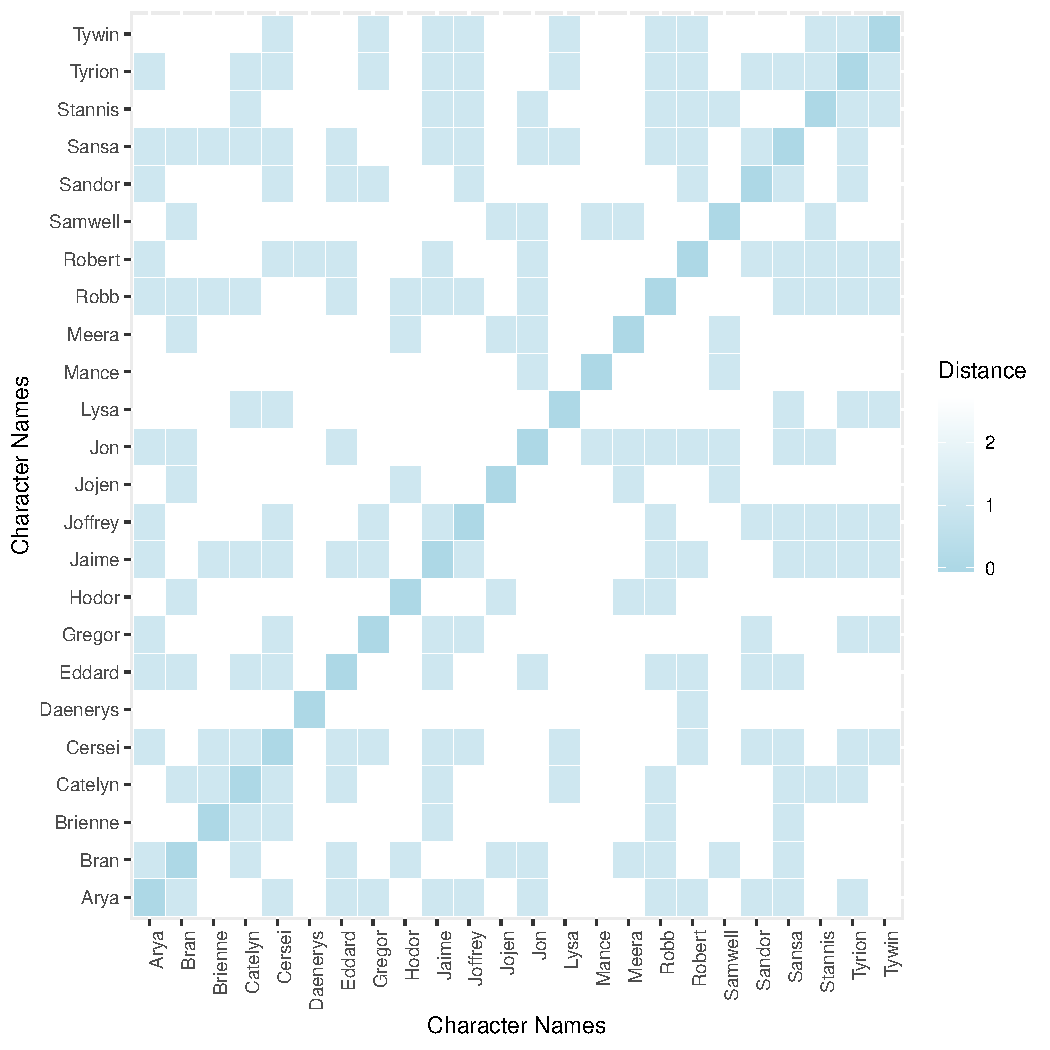
\includegraphics[width = .4\textwidth]{heatmap_dist_unweighted.pdf}
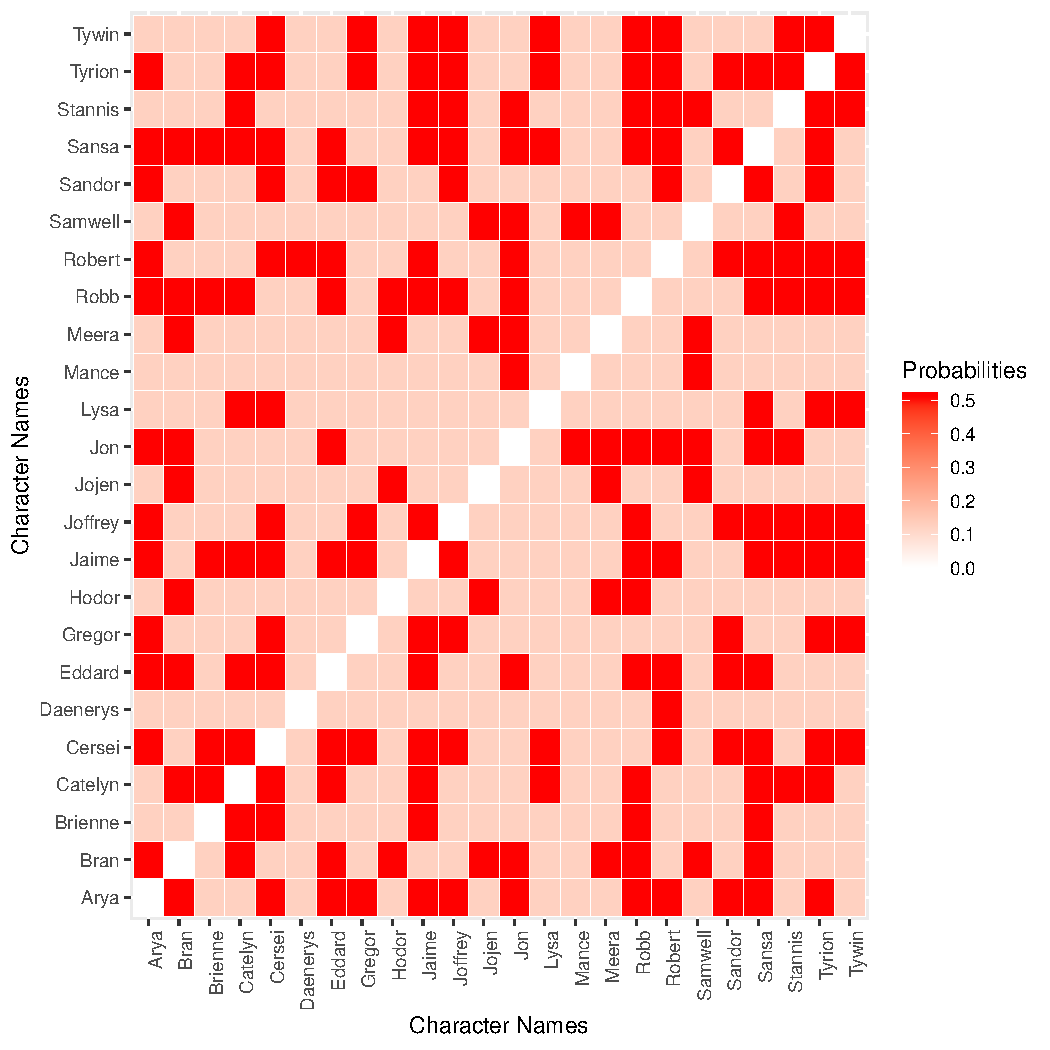
\includegraphics[width = .4\textwidth]{heatmap_p_unweighted.pdf}
\end{center}

The first heat map is constructed using the latent distances and the darker the color, the closer the characters are. The second heat map is constructed using the probabilities of edges between characters, and again, the darker the color, the higher the probability of an edge between the characters. From these heat maps, we do see that some close relationships, like Bran and Hodor, are picked up in both cases. However, it is important to note that in this unweighted model, there is a one-to-one relationship between the latent distances and the presence of an edge and so the EM algorithm only provides estimates of probabilities and distances for when there is an edge and when there isn't an edge between the characters. Thus, we see that these results can be improved.

To this end, we looked to improve this model with the inclusion of the edge weights into our modeling procedure. Following a quite similar approach to that of the unweighted EM algorithm, we use conjugate family relations and Network-Raphson to fit a model that assumes the edge weights follow a Poisson distribution with a parameter we interpret as a function of the distance in the latent space. The results for this analysis follow.
\begin{center}\label{heatmap_weighted}
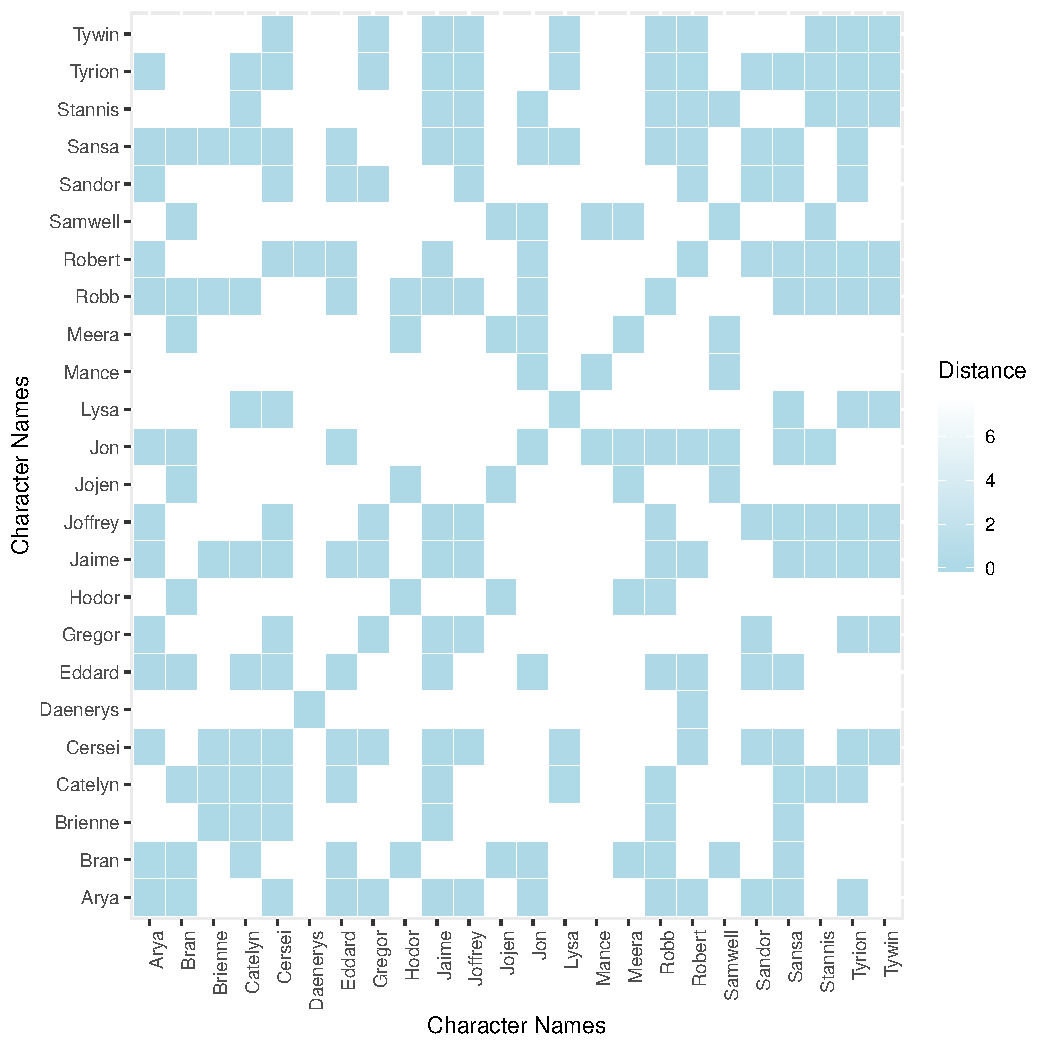
\includegraphics[width = .4\textwidth]{heatmap_dist_weighted.pdf}
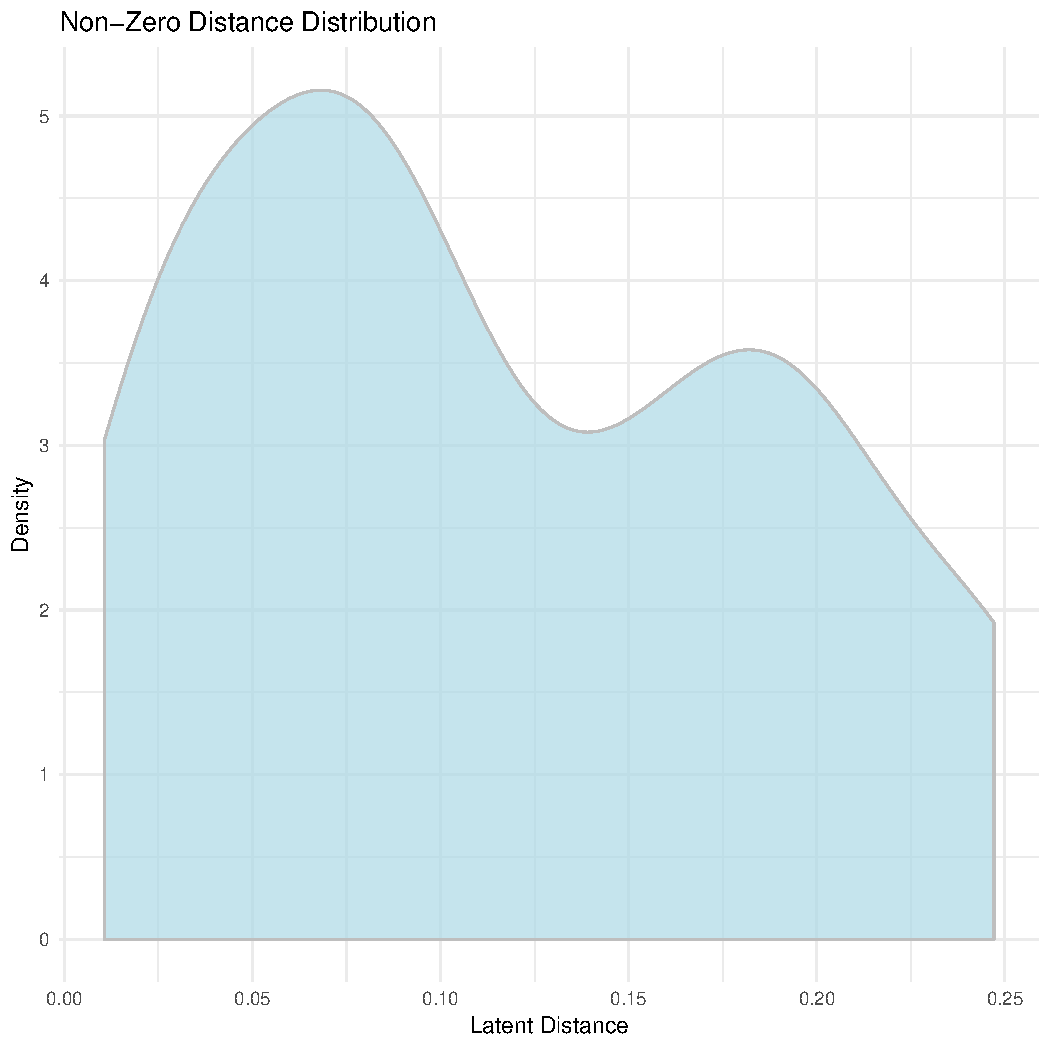
\includegraphics[width = .4\textwidth]{density_dist_weighted.pdf}
\end{center}
The heatmap in the leftmost panel of Figure \ref{heatmap_weighted} is that of the distances between nodes in the network. Lighter squares suggest the vertices are further away while the darker squares represent the vertices are closer. While it appears that this model again only fits a binary relation to the set of distances, we actually see that for those vertices that are ``close'' that this is not the case. Upon investigation of these values, we see that for vertices that do not share an edge, the distance was fit to be near $7$. In essence, this value represents a ``maximal'' distance between vertices. However, for vertices that are not this maximal distance apart, we see that the model is fitting different distances among the vertices. This is evident by the kernel density estimate in the rightmost panel of this figure. Here we see that for distances that are not maximal, the distances between vetices fall in $[0,.25]$ and perhaps come from a smooth bimodal distribution.


In addition to these distances, we provide a similar heatmap in Figure \ref{weighted_clustering} that plots the estimates mean of the Poisson random variable associated with the edge connecting the characters. Darker squares suggest that the number of interactions between the characters is higher and lighter squares represent these characters have less relation. This plot makes clear that this weighted-EM algorithm does appear to detect the number of edges in the network. 


\begin{center}\label{weighted_clustering}
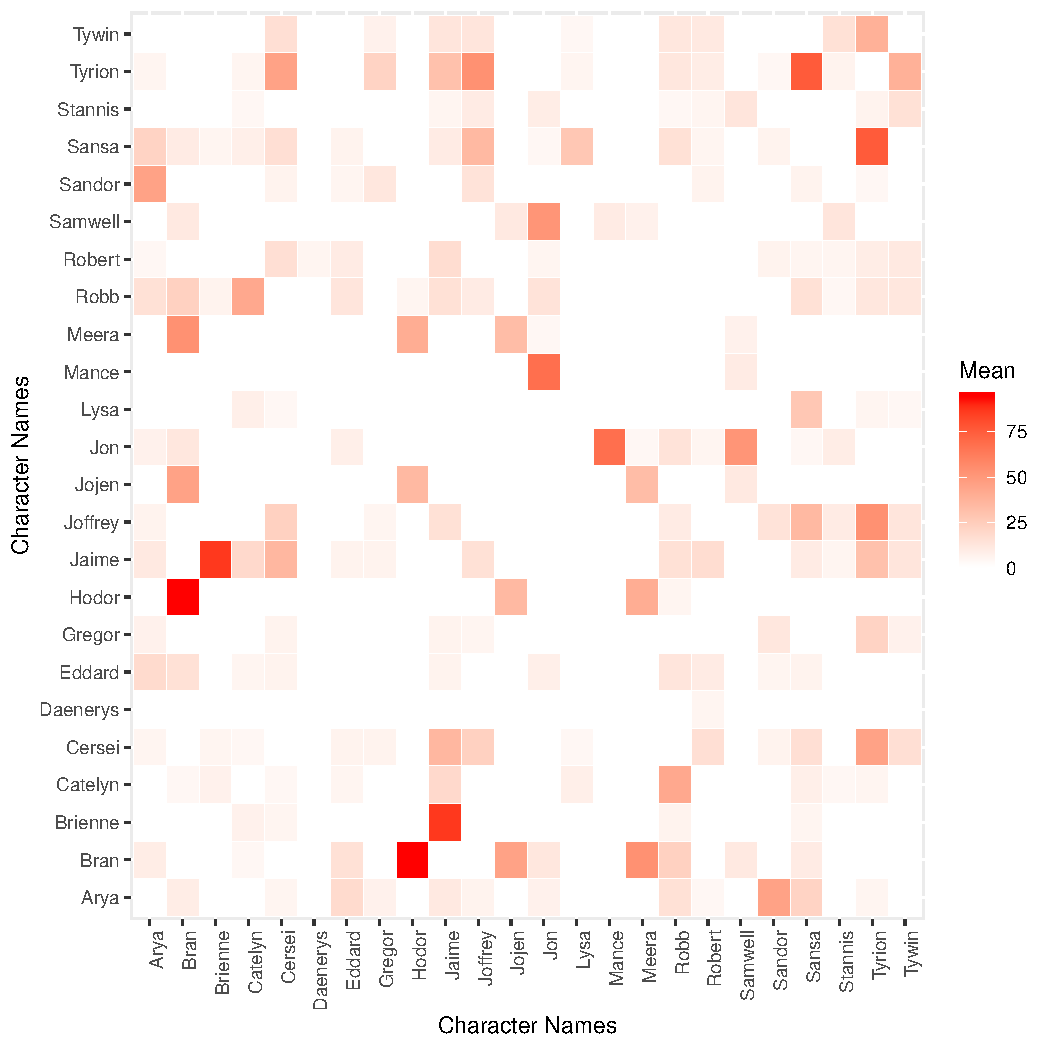
\includegraphics[width = .4\textwidth]{heatmap_p_weighted.pdf}
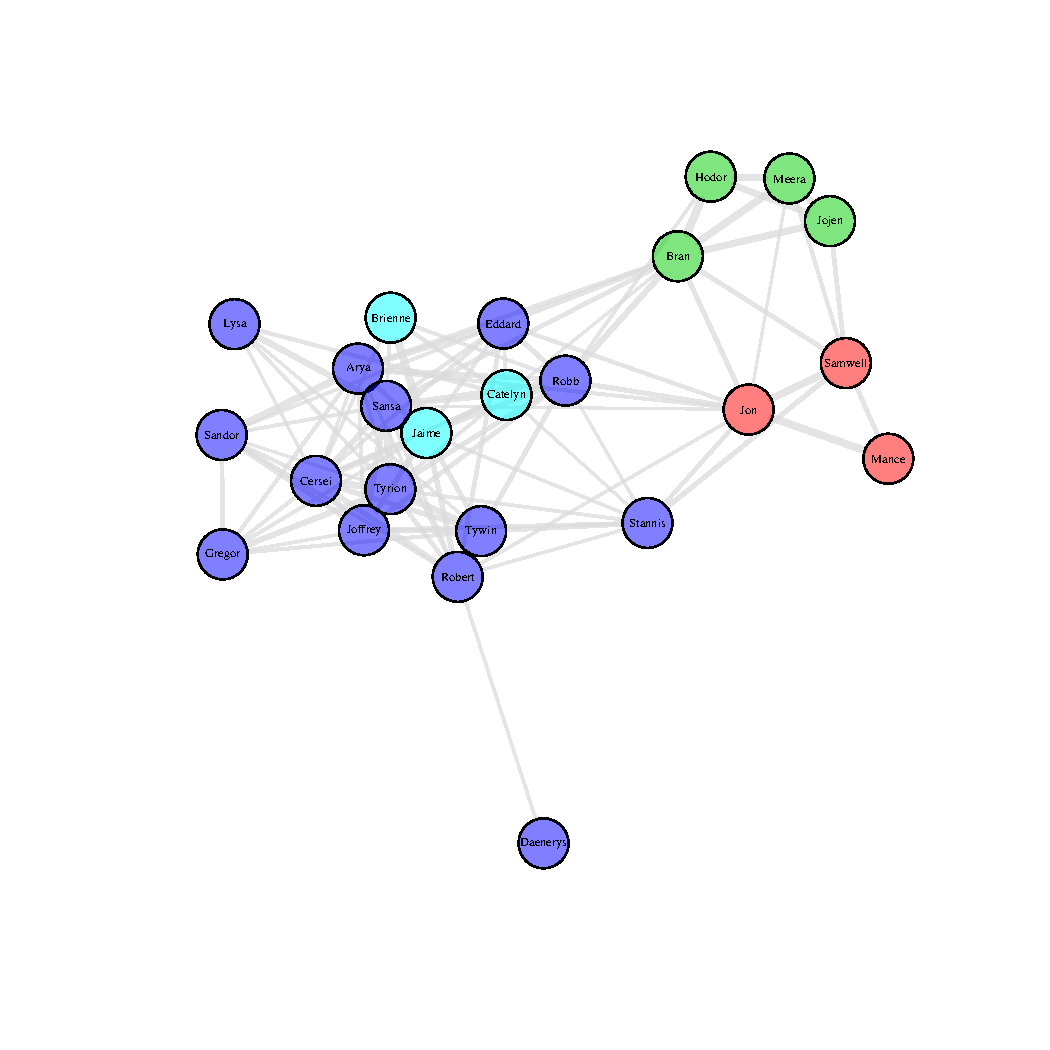
\includegraphics[width = .4\textwidth]{graph_p_clust_weighted.pdf}
\end{center}

As it appears that this model varies more smoothly over the network and accurately reflects the features of the network, we use these estimates for inference tasks. Regarding the estimates provided by the weighted EM algorithm, $\widehat{\Lambda} = [\hat{\lambda}_{ij}]$, as a smoothed, weighted adjacency matrix, we complete spectral clustering as suggested by \cite{Ng:2001:SCA:2980539.2980649}. The results of this cluster analysis can be found in the rightmost panel of Figure \ref{weighted_clustering}. 

 

\subsection{MCMC}

We applied our MCMC algorithm to the model given in Section \ref{MCMC} using $ns = 50000$. Furthermore, we burned the first $20000$ samples and thinned by only taking every tenth sample in the chain. This is consistent with how Hoff used MCMC on Sampson's monk dataset. Additionally, we used $d = 2$ so that our latent variables $Z_i \in \mathbb{R}^2$, and $Nk = 3$, indicating three underlying groups. Assessing the convergence was nontrivial. We determined that our chain was probably not long enough as the group assignments did not meaningfully converge for all characters. We note that our sampling mechanism in the MH step deviates from Hoff's block updates. Consequently, we are ignoring vertex dependencies that are limiting our sampling efficiency. Furthermore, Sampson's monk dataset is represented as a network with fewer actors that our network, so we expect bigger networks will converge more slowly.


We plot the results of our latent variables $Z_i$, as well as the network labeled with the mode of the group assignments in Figure \ref{MCMC_figs}. The means $\mu_k$ for $k \in \{1, 2, 3\}$ are also included in the latent variable embedding plot on th left. Here, we see that the mode does not necessarily correspond to the closest distribution. Nevertheless, we see the group assignments in the network on the right. Six of the characters in green are from the Stark family, while the other two, Samwell and Meera, have close relationships with members of the Stark family. The only Stark not colored green is Jon [Snow], who we later discover is actually not the son of Eddard (Ned) Stark. It is interesting that our method kept him out of the Stark cluster, though that may also be due to his geographical separation from the rest of the family.

\begin{center}\label{MCMC_figs}
\includegraphics[width = .4\textwidth]{{Latent_Embedding_1.0}.pdf}
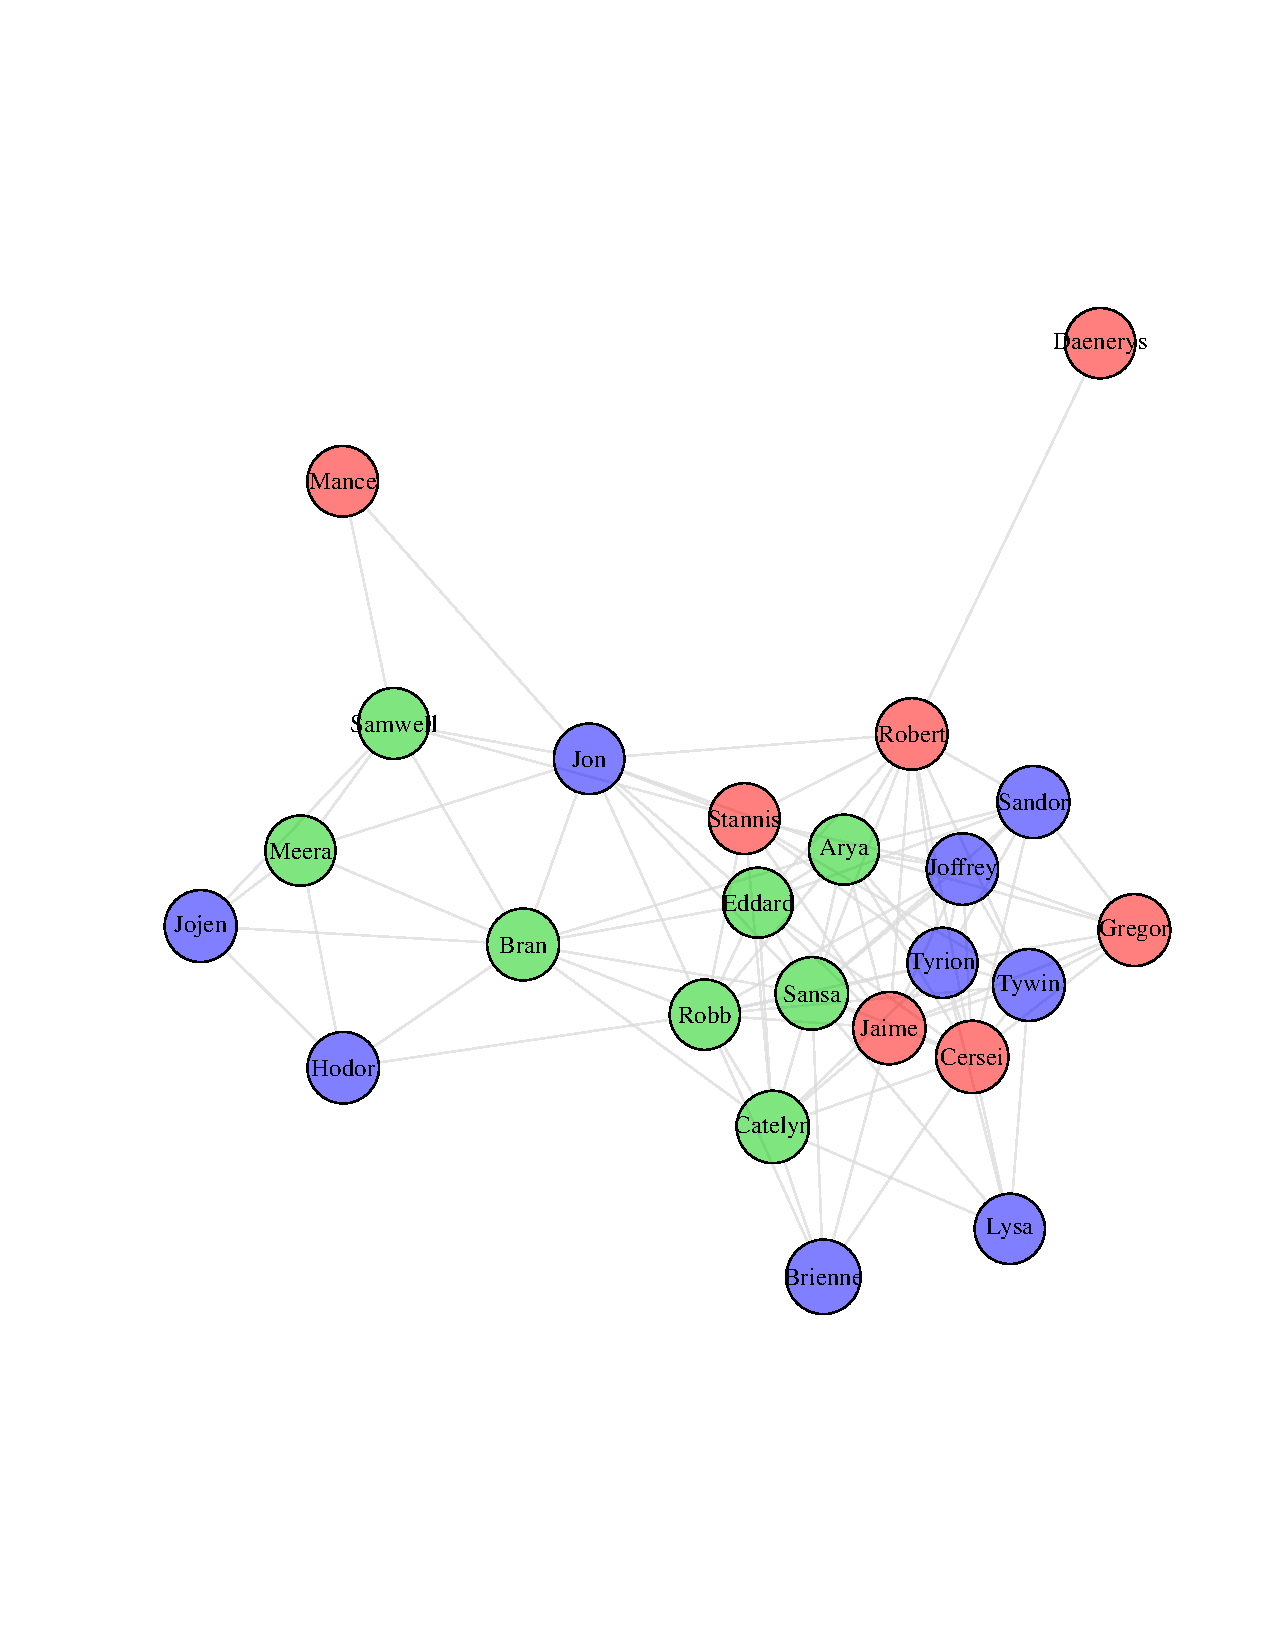
\includegraphics[width = 0.5\textwidth]{Graph_P_Clustering_MCMC.pdf}
\end{center}


\section{Conclusion} \label{Conclusion}

It is clear from this work that latent network models are a useful tool for drawing inferences about a network. In this project, we demonstrate their utility despite the fact that we simplify the model when using EM and neglect block updates with MCMC. We suggest fully following the model development of Hoff for optimal results. Though EM yielded sensible clusters, we are essentially just performing spectral clustering on the observed Laplacian since the weighted EM model is highly parametrized and cannot estimate vertex level latent variables. On the other hand, our MCMC model uses the dichotomized network where an edge is simply any number of interactions, which clearly is a suppression of valuable information. We believe that fitting a Poisson model for the weighted adjacency matrix using MCMC would yield optimal results. Moreover, block updates are probably necessary as our current implementation suffers from ignoring the latent group dependencies. These changes are obvious improvements that should be made.

Additionally, there is a lot of future work that can be accomplished in this area. \textit{A Storm of Swords} is an illustrative choice of books as it is the third and midpoint of all releases, so characters have developed complex relationships. It would be interesting to perform the same analysis across each book and map a character's group status across time. Moreover, there are opportunities to consider the networks from each book as a dynamic network, which is a popular area of research. We hope this project is a nice foundation for future inference on \textit{Game of Thrones} data.

\section{References}
\printbibliography

\newpage
\section*{Appendix}
\appendix 
\section{Estimation Maximization Code}

\lstinputlisting[breaklines=true]{"LNM.EM".R}

\newpage
\section{Markov Chain Monte Carlo Code}

\lstinputlisting{"LNM.MCMC".R}

\end{document}
